% Topic from _Linear Algebra_ Jim Hefferon
%  http://joshua.smcvt.edu/linearalgebra
%  2012-Feb-12
\topic{Magic Squares}
\index{magic square|(}
A Chinese legend tells the story of a  
flood by the Lo river.
People offered sacrifices to appease the river.
Each time a turtle emerged, 
walked around the sacrifice, and returned to the water.
Fuh-Hi, % (2858-2738~BC)
the founder of Chinese civilization,
interpreted this to mean that
the river was still cranky.  
Fortunately, a child noticed 
that on its shell the turtle had the pattern on the left below, which is today
called Lo Shu (``river scroll'').
\begin{center}
  \vcenteredhbox{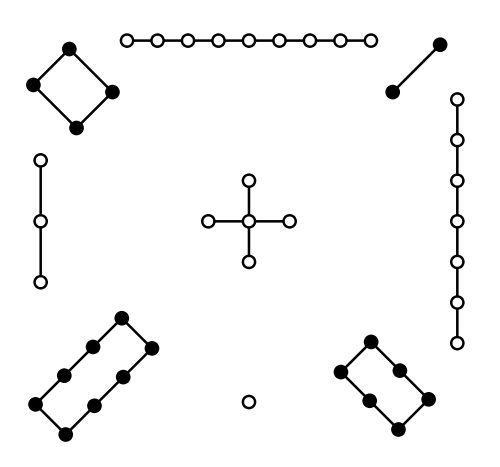
\includegraphics[height=.8in]{LoShu.png}} % http://en.wikipedia.org/wiki/File:Lo_Shu_3x3_magic_square.svg
  \hspace{.8in}
  \begin{tabular}{|c|c|c|}
    \hline
      $4$  &$9$  &$2$  \\ \hline
      $3$  &$5$  &$7$  \\ \hline
      $8$  &$1$  &$6$  \\ \hline    
  \end{tabular}
\end{center}
The dots make the matrix on the right where the
rows, columns, 
and diagonals add to $15$.
Now that the people knew how much to sacrifice, 
the river's anger cooled.
% (http://en.wikipedia.org/wiki/Lo_Shu_Square)

A square matrix is 
\definend{magic}\index{matrix!magic square}\index{magic square!definition}
if each row, column, and diagonal add to the same
number, the matrix's \definend{magic number}.

Another magic square appears in the engraving
\textit{Melencolia I} by D\"urer.
% (http://en.wikipedia.org/wiki/Melencolia_I)
\begin{center}
  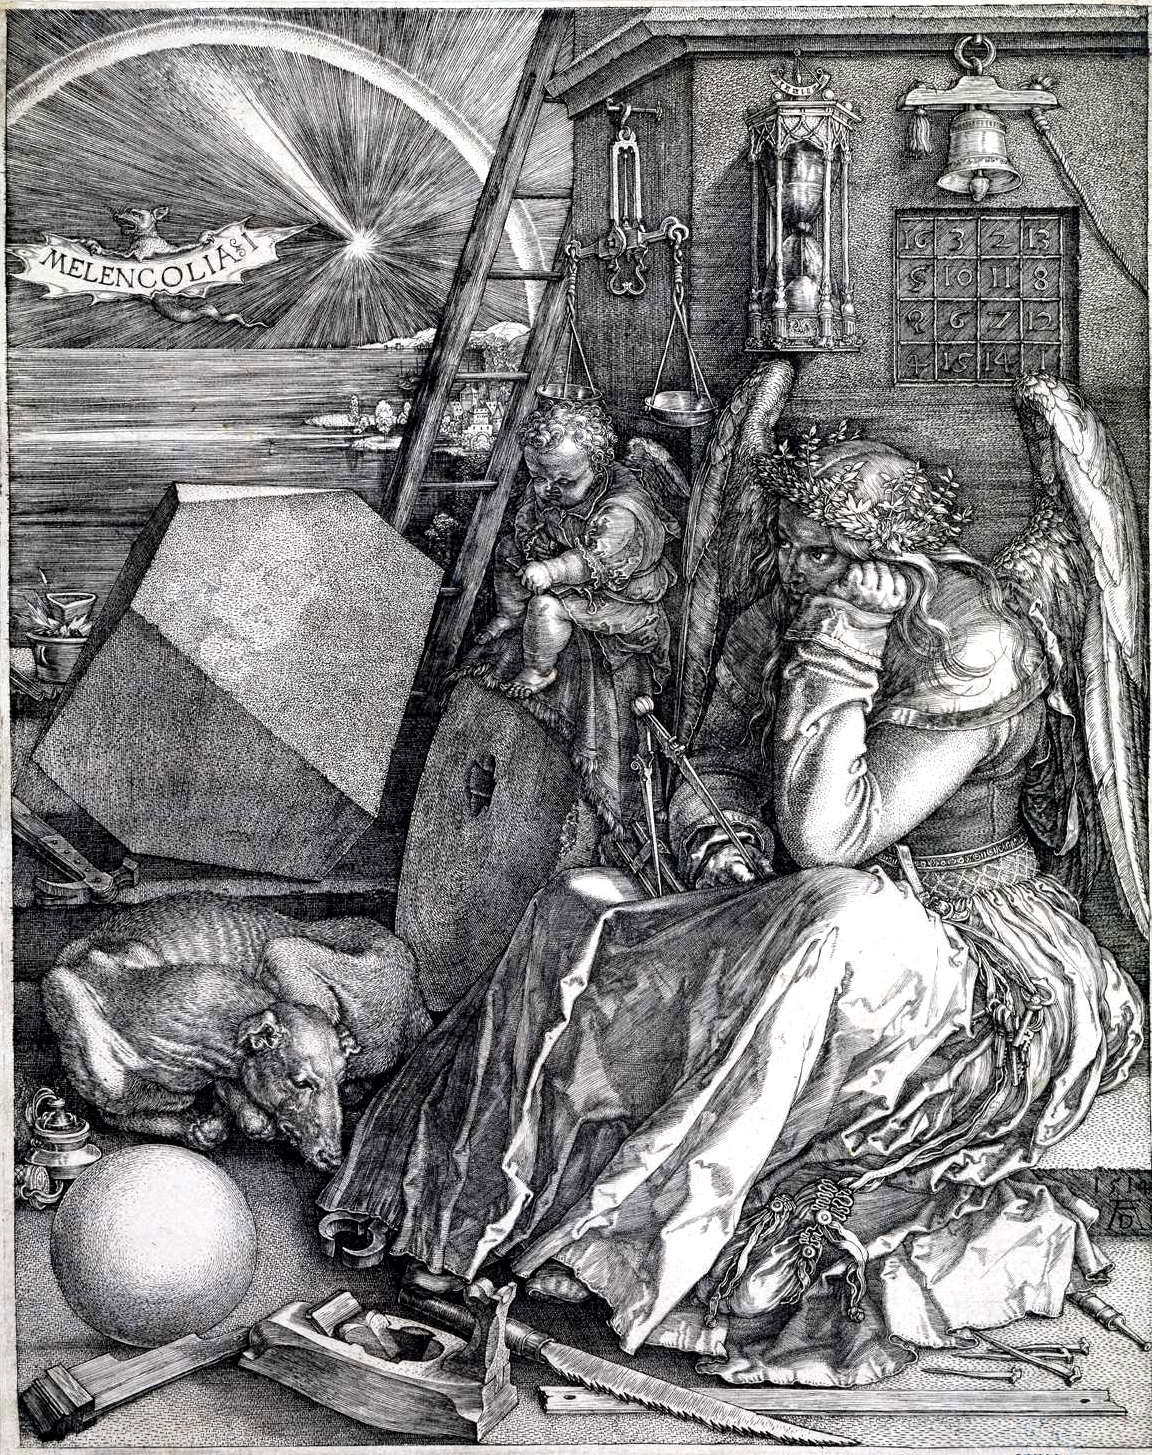
\includegraphics[height=2.20in]{Melencolia.jpg} % wikipedia http://upload.wikimedia.org/wikipedia/commons/1/14/Melencolia_I_%28Durero%29.jpg
\end{center}
One interpretation is that it depicts melancholy, a depressed state.
The figure, genius,
has a wealth of fascinating things to explore including
the compass, the geometrical solid, the scale, and the hourglass.
But the figure is unmoved; all of the things lie unused.
One of the potential delights, in the upper right,
is a $\nbyn{4}$ matrix whose
rows, columns, and diagonals add to~$34$.
\begin{center}
  \vcenteredhbox{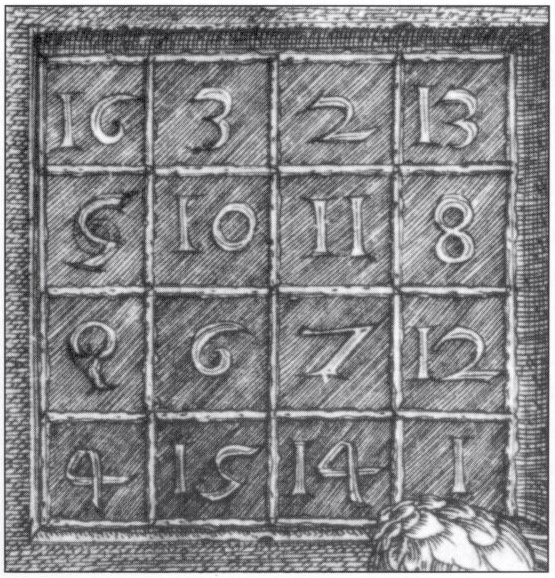
\includegraphics[height=1.25in]{Melencoliadetail.jpg}} % wikipedia http://upload.wikimedia.org/wikipedia/commons/7/7e/Albrecht_D%C3%BCrer_-_Melencolia_I_%28detail%29.jpg
  \hspace{.8in}
  \begin{tabular}{|c|c|c|c|}
    \hline
      $16$  &$3$  &$2$  &$13$  \\ \hline
      $5$   &$10$ &$11$ &$8$   \\ \hline
      $9$   &$6$  &$7$  &$12$  \\ \hline    
      $4$   &$15$ &$14$ &$1$  \\ \hline  
  \end{tabular}
\end{center}
The middle entries on the bottom row give $1514$, the 
date of the engraving.

The above two squares are arrangements of $\interval{1}{n^2}$.
They are \definend{normal}\index{magic square!normal}.
The $\nbyn{1}$ square whose sole entry is $1$ is normal, 
\nearbyexercise{exer:TwoByTwoMagicSqUnique} shows that there is
no normal $\nbyn{2}$ magic square,
and there are normal magic squares of every other size; 
see \cite{WikipediaMagicSquare}.
Finding how many normal magic squares there are of each size is an unsolved
problem;
see \cite{OnlineEncyclopedia}.
 
If we don't require that the squares be normal then we can say much more.
Every $\nbyn{1}$ square is magic, trivially.
If the rows, columns, and diagonals of a $\nbyn{2}$ matrix 
\begin{equation*}
  \begin{mat}
    a  &b  \\
    c  &d
  \end{mat}
\end{equation*}
add to~$s$
then $a+b=s$, $c+d=s$, $a+c=s$, $b+d=s$, $a+d=s$, and $b+c=s$.
\nearbyexercise{exer:TwoByTwoMagicSqUnique} shows that this
system has the unique solution $a=b=c=d=s/2$.
So the set of $\nbyn{2}$ magic squares
is a one-dimensional subspace of $\matspace_{\nbyn{2}}$.

A sum of two same-sized magic squares is magic and a 
scalar multiple of a magic square is magic so the set of 
$\nbyn{n}$ magic squares
$\magicsquares_n$ is a vector space, a subspace of $\matspace_{\nbyn{n}}$.
This Topic shows that for $n\geq 3$ the 
dimension of
$\magicsquares_n$ is $n^2-n$.
The set $\magicsquares_{n,0}$ of $\nbyn{n}$~magic squares with magic number~$0$ 
is another subspace and we will verify the formula for its dimension also:
$n^2-2n-1$ when $n\geq 3$.

We will first prove that $\dim\magicsquares_n=\dim\magicsquares_{n,0}+1$.
Define the 
\definend{trace}\index{trace}\index{matrix!trace} of a matrix to be
the sum down its upper-left to lower-right diagonal
$\trace (M)=m_{1,1}+\cdots+m_{n,n}$.
Consider the restriction of the trace to the magic squares
$\map{\trace}{\magicsquares_n}{\Re}$. 
The null space $\nullspace{\trace}$ is the set of magic squares with magic
number zero 
$\magicsquares_{n,0}$.
Observe that the trace is onto because for any~$r$ in the 
codomain $\Re$ the $\nbyn{n}$ matrix whose entries are all $r/n$ is
a magic square with magic number~$r$.
Theorem~Two.II.\ref{th:RankPlusNullEqDim} says that for any linear map the
dimension of the domain equals the dimension of the range space 
plus the dimension of the null space,
the map's rank plus its nullity.
Here the domain is $\magicsquares_n$, the range space is 
$\Re$ and the null space is $\magicsquares_{n,0}$,
so we have that $\dim\magicsquares_n=1+\dim\magicsquares_{n,0}$.

We will finish by finding the dimension of the vector space
$\magicsquares_{n,0}$. 
For $n=1$ the dimension is clearly $0$.
\nearbyexercise{exer:DimTwoMagicSqsMagicSumZero} shows 
that $\dim\magicsquares_{n,0}$ is also $0$
for $n=2$.

That leaves showing that   
$\dim\magicsquares_{n,0}=n^2-2n-1$ for $n\geq 3$. 
The fact that the squares in this vector space are magic 
gives us a linear system of restrictions, and the 
fact that they have magic number zero makes this system homogeneous: for 
instance consider the $\nbyn{3}$ case.
The restriction that the rows, columns, and diagonals of 
\begin{equation*}
    \begin{mat}
      a &b &c \\
      d &e &f \\
      g &h &i
    \end{mat}
\end{equation*}
add to zero gives this $\nbym{(2n+2)}{n^2}$ linear system.
\begin{equation*}
  \begin{linsys}{9}
    a &+ &b &+ &c &  &  &  &  &  &  &  &  &  &  &  &  &= &0 \\ 
      &  &  &  &  &  &d &+ &e &+ &f &  &  &  &  &  &  &= &0 \\ 
      &  &  &  &  &  &  &  &  &  &  &  &g &+ &h &+ &i &= &0 \\ 
    a &  &  &  &  &+ &d &  &  &  &  &+ &g &  &  &  &  &= &0 \\ 
      &  &b &  &  &  &  &+ &e &  &  &  &  &+ &h &  &  &= &0 \\ 
      &  &  &  &c &  &  &  &  &+ &f &  &  &  &  &+ &i &= &0 \\ 
    a &  &  &  &  &  &  &+ &e &  &  &  &  &  &  &+ &i &= &0 \\ 
      &  &  &  &c &  &  &+ &e &  &  &+ &g &  &  &  &  &= &0    
  \end{linsys}
\end{equation*}
We will find the dimension of the space by finding the number of 
free variables in the linear system.

The matrix of coefficients for the particular cases of $n=3$ and~$n=4$
are below, with the rows and columns numbered to help in reading
the proof.
With respect to the standard basis, each represents a linear map
$\map{h}{\Re^{n^2}}{\Re^{2n+2}}$.
The domain has dimension~$n^2$ so if we show that the
rank of the matrix is $2n+1$ then we will have
what we want, that the dimension of the null space 
$\magicsquares_{n,0}$ is $n^2-(2n+1)$.
\newlength{\interblockhspace}
\setlength{\interblockhspace}{1.45em}
\newlength{\interblockvspace}
\setlength{\interblockvspace}{1ex}
\newlength{\colwidth}
\settowidth{\colwidth}{$9$}
\begin{equation*}
  \begin{array}{r|ccc@{\hspace*{\interblockhspace}}ccc@{\hspace*{\interblockhspace}}ccc}
    \multicolumn{1}{c}{\ }  &1 &2 &3 &4 &5 &6 &7 &8 &9 \\
    \cline{2-10}
    \vec{\rho}_1 &1 &1 &1 &0 &0 &0 &0 &0 &0 \\
    \vec{\rho}_2 &0 &0 &0 &1 &1 &1 &0 &0 &0 \\
    \vec{\rho}_3 &0 &0 &0 &0 &0 &0 &1 &1 &1 \\[\interblockvspace]
    \vec{\rho}_4 &1 &0 &0 &1 &0 &0 &1 &0 &0 \\
    \vec{\rho}_5 &0 &1 &0 &0 &1 &0 &0 &1 &0 \\
    \vec{\rho}_6 &0 &0 &1 &0 &0 &1 &0 &0 &1 \\[\interblockvspace]
    \vec{\rho}_7 &1 &0 &0 &0 &1 &0 &0 &0 &1 \\
    \vec{\rho}_8 &0 &0 &1 &0 &1 &0 &1 &0 &0 
  \end{array}
\end{equation*}
\begin{equation*}
  \begin{array}{r|cccc@{\hspace*{\interblockhspace}}cccc@{\hspace*{\interblockhspace}}cccc@{\hspace*{\interblockhspace}}cccc}
    \multicolumn{1}{c}{\ }  &1 &2 &3 &4 &5 &6 &7 &8 &9 
           &\makebox[\colwidth]{$10$} &\makebox[\colwidth]{$11$} 
           &\makebox[\colwidth]{$12$} &\makebox[\colwidth]{$13$} 
           &\makebox[\colwidth]{$14$} &\makebox[\colwidth]{$15$} 
           &\makebox[\colwidth]{$16$} \\
    \cline{2-17}
    \vec{\rho}_1   &1 &1 &1 &1  &0 &0 &0 &0  &0 &0 &0 &0  &0 &0 &0 &0 \\
    \vec{\rho}_2   &0 &0 &0 &0  &1 &1 &1 &1  &0 &0 &0 &0  &0 &0 &0 &0 \\
    \vec{\rho}_3   &0 &0 &0 &0  &0 &0 &0 &0  &1 &1 &1 &1  &0 &0 &0 &0 \\
    \vec{\rho}_4   &0 &0 &0 &0  &0 &0 &0 &0  &0 &0 &0 &0  &1 &1 &1 &1 \\[\interblockvspace]
    \vec{\rho}_5   &1 &0 &0 &0  &1 &0 &0 &0  &1 &0 &0 &0  &1 &0 &0 &0 \\
    \vec{\rho}_6   &0 &1 &0 &0  &0 &1 &0 &0  &0 &1 &0 &0  &0 &1 &0 &0 \\
    \vec{\rho}_7   &0 &0 &1 &0  &0 &0 &1 &0  &0 &0 &1 &0  &0 &0 &1 &0 \\
    \vec{\rho}_8   &0 &0 &0 &1  &0 &0 &0 &1  &0 &0 &0 &1  &0 &0 &0 &1 \\[\interblockvspace]
    \vec{\rho}_9   &1 &0 &0 &0  &0 &1 &0 &0  &0 &0 &1 &0  &0 &0 &0 &1 \\
    \vec{\rho}_{10} &0 &0 &0 &1  &0 &0 &1 &0  &0 &1 &0 &0  &1 &0 &0 &0 \\
  \end{array}
\end{equation*}

We want to show that the rank of the matrix of coefficients,
the number of rows in a maximal linearly independent set, is $2n+1$.
The first $n$~rows of the matrix of coefficients add to the same vector
as the second $n$~rows, the vector of all ones.
So a maximal linearly independent must omit at least one row.
We will show that the set of all rows but the first 
$\setinterval{\vec{\rho}_2}{\vec{\rho}_{2n+2}}$
is linearly independent.
So consider this linear relationship.
\begin{equation*}
  c_2\vec{\rho}_2+\cdots+c_{2n}\vec{\rho}_{2n}
     +c_{2n+1}\vec{\rho}_{2n+1}+c_{2n+2}\vec{\rho}_{2n+2}=\zero
   \tag{$*$}
\end{equation*}

Now it gets messy.
Focus on the lower left of the tables.
Observe that in the final two rows, in the first~$n$ columns, is a subrow that 
is all zeros except that it starts with a one in column~$1$
and a subrow that is all zeros except that it ends with a one
in column~$n$.

First, with $\vec{\rho}_1$ omitted, both column~$1$ and column~$n$ contain only 
two ones.
Since the only rows in~($*$) with nonzero column~$1$ entries 
are rows $\vec{\rho}_{n+1}$ and $\vec{\rho}_{2n+1}$, which have ones, 
we must have $c_{2n+1}=-c_{n+1}$.
Likewise considering the $n$-th entries of the vectors in~($*$) gives that
$c_{2n+2}=-c_{2n}$.

Next consider the columns between those two\Dash
in the $n=3$ table this includes only column~$2$ while 
in the $n=4$~table it includes both columns~$2$ and~$3$.
Each such column has a single one.
That is, for each column index $j\in\setinterval{2}{n-2}$
the column consists of only zeros except for a one in row~$n+j$, 
and hence $c_{n+j}=0$.

On to the next block of columns, from $n+1$ through~$2n$.
Column~$n+1$ has only two ones (because $n\geq 3$ the ones
in the last two rows do not fall in the first column of this
block). 
Thus $c_2=-c_{n+1}$
and therefore $c_2=c_{2n+1}$.
Likewise, from column~$2n$ we conclude that $c_2=-c_{2n}$
and so $c_2=c_{2n+2}$.  

Because $n\geq 3$
there is at least one column between column~$n+1$ and column~$2n-1$.
In at least one of those columns a one appears in $\vec{\rho}_{2n+1}$.
If a one also appears in that column in $\vec{\rho}_{2n+2}$ then we have 
$c_2=-(c_{2n+1}+c_{2n+2})$ 
since $c_{n+j}=0$ for $j\in\setinterval{2}{n-2}$.
If a one does not appear in that column in $\vec{\rho}_{2n+2}$
then we have $c_2=-c_{2n+1}$.
In either case $c_2=0$, and thus 
$c_{2n+1}=c_{2n+2}=0$ and  
$c_{n+1}=c_{2n}=0$.

If the next block of $n$-many columns is not the last then similarly
conclude from its 
first column that $c_3=c_{n+1}=0$.

Keep this up until we reach the last block of columns, those numbered
$(n-1)n+1$ through~$n^2$.
Because $c_{n+1}=\cdots=c_{2n}=0$ column~$n^2$ 
gives that $c_{n}=-c_{2n+1}=0$.

Therefore the rank of the matrix is $2n+1$, as required.

\medskip
The classic source on normal magic squares is \cite{Ball}.
More on the Lo Shu square is at \cite{WikipediaLoShuSquare}.
The proof given here began with \cite{Ward}.

\begin{exercises}
  \item Let $M$ be a $\nbyn{3}$ magic square with magic number~$s$.
    \begin{exparts}
      \partsitem Prove that the sum of $M$'s entries is $3s$.
      \partsitem Prove that $s=3\cdot m_{2,2}$.
      \partsitem Prove that $m_{2,2}$ is the average of the entries
        in its row, its column, and in each diagonal.
      \partsitem Prove that $m_{2,2}$ is the median of $M$'s entries.
    \end{exparts}
    \begin{answer}
      \begin{exparts}
        \partsitem The sum of the entries of $M$ is the sum of the sums of
          the three rows. 
        \partsitem The constraints on entries of $M$ involving the center 
          entry make this system.
          \begin{equation*}
            \begin{linsys}{3}
              m_{2,1}  &+  &m_{2,2}  &+  &m_{2,3}  &=  &s  \\ 
              m_{1,2}  &+  &m_{2,2}  &+  &m_{3,2}  &=  &s  \\ 
              m_{1,1}  &+  &m_{2,2}  &+  &m_{3,3}  &=  &s  \\ 
              m_{1,3}  &+  &m_{2,2}  &+  &m_{3,1}  &=  &s  
            \end{linsys}
          \end{equation*}
          Adding those four equations counts each matrix entry once and only
          once, except that we count the center entry four times.
          Thus the left side sums to $3s+3m_{2,2}$ while the right sums to $4s$.
          So $3m_{2,2}=s$.
        \partsitem
          The second row adds to $s$ so $m_{2,1}+m_{2,2}+m_{2,3}=3m_{2,2}$,
          giving that $(1/2)\cdot(m_{2,1}+m_{2,3})=m_{2,2}$.
          The same goes for the column and the diagonals.
        \partsitem
          By the prior exercise either both $m_{2,1}$ and $m_{2,3}$ are equal
          to $m_{2,2}$ or else one is greater while one is smaller.
          Thus $m_{2,2}$ is the median of the set
          $\set{m_{2,1},m_{2,2},m_{2,3}}$.
          The same reasoning applied to the second column shows that 
          Thus $m_{2,2}$ is the median of the set
          $\set{m_{1,2},m_{2,1},m_{2,2},m_{2,3},m_{3,2}}$.
          Extending to the two diagonals shows it is the median of the set
          of all entries.
      \end{exparts}
    \end{answer}
  \item \label{exer:TwoByTwoMagicSqUnique}
    Solve the system $a+b=s$, $c+d=s$, $a+c=s$, $b+d=s$, $a+d=s$, and $b+c=s$.
    \begin{answer}
      For any $k$ we have this.
      \begin{multline*}
        \begin{amat}{4}
          1  &1  &0  &0  &s  \\
          0  &0  &1  &1  &s  \\
          1  &0  &1  &0  &s  \\
          0  &1  &0  &1  &s  \\
          1  &0  &0  &1  &s  \\
          0  &1  &1  &0  &s            
        \end{amat}
        \grstep[-\rho_1+\rho_5]{-\rho_1+\rho_3}
        \begin{amat}{4}
          1  &1  &0  &0  &s  \\
          0  &0  &1  &1  &s  \\
          0  &-1 &1  &0  &0  \\
          0  &1  &0  &1  &s  \\
          0  &-1 &0  &1  &0  \\
          0  &1  &1  &0  &s            
        \end{amat}                                            \\
        \grstep{-\rho_2\leftrightarrow\rho_6}
        \begin{amat}{4}
          1  &1  &0  &0  &s  \\
          0  &1  &1  &0  &s  \\          
          0  &-1 &1  &0  &0  \\
          0  &1  &0  &1  &s  \\
          0  &-1 &0  &1  &0  \\
          0  &0  &1  &1  &s  
        \end{amat}
        \grstep[-\rho_2+\rho_4 \\ \rho_2+\rho_5]{-\rho_2+\rho_3}
        \begin{amat}{4}
          1  &1  &0  &0  &s  \\
          0  &1  &1  &0  &s  \\          
          0  &0  &2  &0  &s  \\
          0  &1  &-1 &1  &0  \\
          0  &0  &1  &1  &s  \\
          0  &0  &1  &1  &s  
        \end{amat}
      \end{multline*}
      The unique solution is $a=b=c=d=s/2$.
    \end{answer}
  \item \label{exer:DimTwoMagicSqsMagicSumZero} 
    Show that $\dim\magicsquares_{2,0}=0$.
    \begin{answer}
       By the prior exercise the only member is $Z_{\nbyn{2}}$.
    \end{answer}
  \item   \label{exer:TraceIsLinear}
    Let the \definend{trace} function be 
    $\trace (M)=m_{1,1}+\cdots+m_{n,n}$.
    Define also
    the sum down the other diagonal
    $\trace^* (M)=m_{1,n}+\cdots+m_{n,1}$.
    \begin{exparts}
      \partsitem 
        Show that the two functions 
        $\map{\trace,\trace^*}{\matspace_{\nbyn{n}}}{\Re}$
        are linear.
      \partsitem
        Show that the function
       $\map{\theta}{\matspace_{\nbyn{n}}}{\Re^2}$
       given by $\theta(M)=(\trace(M),\trace^*(m))$
       is linear.
     \partsitem
       Generalize the prior item. 
    \end{exparts}
    \begin{answer}
      \begin{exparts}
        \partsitem
          Where $M,N\in\matspace_{\nbyn{n}}$ we have 
          $\trace(cM+dN)=(cm_{1,1}+dn_{1,1})+\cdots+(cm_{n,n}+dn_{n,n})
          =(cm_{1,1}+\cdots+cm_{n,n})+(dn_{1,1}+\cdots+dn_{n,n})
          =c\cdot\trace(M)+d\cdot\trace(N)$ where
          all numbers are real, so the trace preserves linear
         combinations.
         The argument for $\trace^*$ is similar.
       \partsitem
         It preserves linear combinations: where all numbers are real,
          $\theta(cM+dN)=(\trace(cM+dN),\trace^*(cM+dN))
          =(c\cdot\trace(M)+d\cdot\trace(N), c\cdot\trace^*(M)+d\cdot\trace^*(N))
          =c\cdot\theta(M)+d\cdot\theta(N)$.
       \partsitem   
         Where $\map{h_1,\ldots,h_n}{V}{W}$ are linear then so is
         $\map{g}{V}{W^n}$ given by
         $g(\vec{v})=(h_1(\vec{v}), \ldots, h_n(\vec{v}))$.
         The proof just follows the proof of the prior item.
      \end{exparts}
    \end{answer}
  \item A square matrix is \definend{semimagic} if 
     the rows and columns add to the same value, that is, if we drop the
     condition on the diagonals.
     \begin{exparts*}
       \partsitem
         Show that the set of semimagic squares $\semimagicsquares_n$ 
         is a subspace of $\matspace_{\nbyn{n}}$.
       \partsitem
         Show that 
         the set $\semimagicsquares_{n,0}$  
         of $\nbyn{n}$~semimagic squares with magic number~$0$
         is also a subspace of $\matspace_{\nbyn{n}}$.
     \end{exparts*}
     \begin{answer}
       \begin{exparts*}
         \partsitem
           The sum of two semimagic squares is semimagic, as is a scalar 
           multiple of a semimagic square.
         \partsitem
           As with the prior item, a linear combination of two semimagic
           squares with magic number zero is also such a matrix.
       \end{exparts*}
     \end{answer}
  \item 
    \cite{Beardon}
    Here is a slicker proof of the result of this Topic, when $n\geq 3$.
    See the prior two exercises for some definitions and needed results.
    \begin{exparts}
      \partsitem
        First show that 
        $\dim\magicsquares_{n,0}=\dim\semimagicsquares_{n,0}+2$.
        To do this, consider the function
        $\map{\theta}{\matspace_n}{\Re^2}$ sending a 
        matrix~$M$ to
        the ordered pair $(\trace(M),\trace^*(M))$.
        Specifically, consider the restriction of that map
        $\map{\theta}{\semimagicsquares_n}{\Re^2}$ to the semimagic squares.  
        Clearly its null space is $\magicsquares_{n,0}$.
        Show that when $n\geq 3$ this restriction $\theta$ is onto.
        (\textit{Hint:} we need only find a basis for 
           $\Re^2$ that is the
           image of two members of $\mathcal{H}_n$)  
      \partsitem
        Let the function $\map{\phi}{\matspace_{\nbyn{n}}}{\matspace_{\nbyn{(n-1)}}}$
        be the identity map except that it 
        drops the final row and column: $\phi(M)=\hat{M}$ where 
        $\hat{m}_{i,j}=m_{i,j}$ for all $i,j\in\setinterval{1}{n-1}$.
        The check that $\phi$ is linear is easy.
        Consider $\phi$'s restriction to the semimagic squares with 
        magic number zero
       $\map{\phi}{\semimagicsquares_{n,0}}{\matspace_{\nbyn{(n-1)}}}$.
       Show that $\phi$ is one-to-one
     \partsitem
       Show that $\phi$ is onto.
     \partsitem Conclude that
        $\semimagicsquares_{n,0}$ has dimension~$(n-1)^2$.
     \partsitem 
        Conclude that $\dim(\magicsquares_n)=n^2-n$
    \end{exparts}
    \begin{answer}
      \begin{exparts}
        \partsitem
          Consider the matrix $C\in \mathcal{H}_n$ that has all 
          entries zero except
          that the four corners are $c_{1,1}=c_{n,n}=1$ and $c_{1,n}=c_{n,1}=-1$.
           Also consider the matrix $D\in \mathcal{H}_n$ with all entries 
           zero except that 
           $d_{1,1}=d_{2,2}=1$ and $d_{1,2}=d_{2,1}=-1$.
           We have
           \begin{equation*}
              \theta(C)=\colvec{2 \\ -2}
              \qquad
              \theta(D)=\begin{cases}
                           \binom{2}{-1}  &\text{if $n=3$}  \\[1ex]
                           \binom{2}{0}  &\text{if $n>3$}
                        \end{cases}
           \end{equation*}
           and so the image of $\theta$ includes a basis for $\Re^2$ and
           thus $\theta$ is onto.
           With that, because for any linear map the
           dimension of the domain equals its rank plus its nullity
           we conclude that 
           $\dim(\mathcal{H}_n)=2+\dim(\magicsquares_{n,0})$, as desired.
        \partsitem
           We claim that 
           $\map{\phi}{\semimagicsquares_{n,0}}{\matspace_{\nbyn{(n-1)}}}$.
           is one-to-one and onto.

           To show that it is one-to-one we will show that the only member of 
           $\semimagicsquares_{n,0}$ mapped to the zero matrix $Z_{\nbyn{(n-1)}}$
           is the zero matrix~$Z_{\nbyn{n}}$.
           Suppose that $M\in\semimagicsquares_{\nbyn{n}}$ and 
           $\phi(M)=Z_{\nbyn{(n-1)}}$.
           On all but the final row and column $\phi$ is the identity so
           the entries in $M$ in all but the final row and column are zero: 
           $m_{i,j}=0$ for $i,j\in\setinterval{1}{n-1}$.
           The first row of $M$ adds to zero and hence
           the final entry in that row $m_{1,n}$ is zero.
           Similarly the final entry in each row $i\in\setinterval{1}{n-1}$
           and column $j\in\setinterval{1}{n-1}$ is zero.
           Then, the final column adds to zero so $m_{n,n}=0$.
           Therefore $M$ is the zero matrix $Z_{\nbyn{n}}$ and the 
           restriction of $\phi$ 
           is one-to-one. 
        \partsitem
           Consider a member $\hat{M}$ of the codomain $\matspace_{\nbyn{(n-1)}}$.
           We will produce a matrix $M$ from the domain 
           $\semimagicsquares_{n,0}$ that maps to it.
           The function $\phi$ is the identity on all but the final row 
           and column of 
           $M$ so for $i,j\in\setinterval{1}{n-1}$
           the entries are $m_{i,j}=\hat{m}_{i,j}$.
           \begin{equation*}
             M=\begin{mat}
               \hat{m}_{1,1}    &\hat{m}_{1,2}  &\ldots &\hat{m}_{1,n-1} &m_{1,n}  \\
               \vdotswithin{\hat{m}_{1,1}}  
                 &\vdotswithin{\hat{m}_{1,2}}     \\
               \hat{m}_{n-1,1}  &\hat{m}_{n-1,2} &\ldots &\hat{m}_{n-1,n-1} &m_{n-1,n}  \\
               m_{n,1}         &m_{n,2}         &\ldots &m_{n,n-1}        &m_{n,n}  
            \end{mat}
          \end{equation*}
          The first row of $M$ must add to zero so we take $m_{1,n}$ to be  
          $-(\hat{m}_{1,1}+\cdots+\hat{m}_{1,n-1})$.
          In the same way we get the final entries 
          $m_{i,n}=-(\hat{m}_{i,1}+\cdots+\hat{m}_{i,n-1})$ in all the rows but the 
          bottom $i\in\setinterval{1}{n-1}$, 
          and the final entries $m_{n,j}=-(\hat{m}_{1,j}+\cdots+\hat{m}_{n-1,j})$ 
          in all the columns but the last
          $j\in\setinterval{1}{n-1}$.
          The entry remaining is the one in the lower right~$m_{n,n}$.
          The final column adds to zero so we set it to 
          $-(m_{1,n}+\cdots+m_{n-1,n})$ but we must check
          that the final row now also adds to zero.
          We have $m_{n,n}=-m_{1,n}-\cdots-m_{n-1,n}$ and expanding each of the
          $m_{i,n}$ as $-\hat{m}_{1,1}-\cdots-\hat{m}_{1,n-1}$
          gives that we have defined $m_{n,n}$ to be the sum of all the entries
          of $\hat{M}$.
          The sum of the all the entries but the last in the final row is
          $m_{1,n}+m_{2,n}+\cdots+m_{n-1,n}$ and expanding each 
          $m_{n,j}=-\hat{m}_{1,j}-\cdots-\hat{m}_{n-1,j}$ 
          verifies that the sum of the final row is zero.
          Thus $M$ is semimagic with magic number zero and so $\phi$ is onto.
        \partsitem
           Theorem~Two.II.\ref{th:RankPlusNullEqDim} says that for any linear 
           map the
           dimension of the domain equals its rank plus its nullity.
           Because $\map{\phi}{\semimagicsquares_n}{\matspace_{\nbyn{(n-1)}}}$ 
           is one-to-one its nullity is zero.
           Because it is onto its rank is $\dim(\matspace_{\nbyn{(n-1)}})=(n-1)^2$.
           Thus the domain of $\phi$, the subspace  
           $\semimagicsquares_{n,0}$ of semimagic squares with magic number zero,
           has dimension~$(n-1)^2$.
         \partsitem   
           We have that $\dim\magicsquares_n=\dim\magicsquares_{n,0}+1
           =(\dim\semimagicsquares_n-2)+1=(n-1)^2-1=n^2-n$ 
           when $n\geq 3$.
      \end{exparts}
    \end{answer}
\end{exercises}
\index{magic square|)}
\endinput


